%==============================================================================
% Sjabloon onderzoeksvoorstel bachproef
%==============================================================================
% Gebaseerd op document class `hogent-article'
% zie <https://github.com/HoGentTIN/latex-hogent-article>

% Voor een voorstel in het Engels: voeg de documentclass-optie [english] toe.
% Let op: kan enkel na toestemming van de bachelorproefcoördinator!
\documentclass{hogent-article}

% Invoegen bibliografiebestand
\addbibresource{voorstel.bib}

% Informatie over de opleiding, het vak en soort opdracht
\studyprogramme{Professionele bachelor toegepaste informatica}
\course{Bachelorproef}
\assignmenttype{Onderzoeksvoorstel}
% Voor een voorstel in het Engels, haal de volgende 3 regels uit commentaar
% \studyprogramme{Bachelor of applied information technology}
% \course{Bachelor thesis}
% \assignmenttype{Research proposal}

\academicyear{2023-2024} 

% TODO: Werktitel
\title{Onderzoek naar het optimale gebruik van Garbage Collection in Java voor migratie naar mainframe.}

\author{Eddy Briké}
\email{eddy.brike@student.hogent.be}


% Gaat het om een bachelorproef in samenwerking met een student in een andere
% opleiding? Geef dan de naam en emailadres hier
% \author{Yasmine Alaoui (naam opleiding)}
% \email{yasmine.alaoui@student.hogent.be}

% TODO: Geef de co-promotor op
\supervisor[Co-promotor]{Jan Cannaerts (Solidaris, \href{mailto:jan.cannaerts@solidaris.be}{jan.cannaerts@solidaris.be})}

% Binnen welke specialisatierichting uit 3TI situeert dit onderzoek zich?
% Kies uit deze lijst:
%
% - Mobile \& Enterprise development
% - AI \& Data Engineering
% - Functional \& Business Analysis
% - System \& Network Administrator
% - Mainframe Expert
% - Als het onderzoek niet past binnen een van deze domeinen specifieer je deze
%   zelf
%
\specialisation{Mainframe Expert}
\keywords{Java, Garbage Collection, Mainframe}

\begin{document}

%TODO: Samenvatting
\begin{abstract}
    
  Garbage Collection is een onderdeel van vershillende programmeertalen, waaronder Java.
  Garbage Collection zorgt ervoor dat geheugen die niet meer wordt gebruikt terug vrij komt.
  Deze onderzoek wil zich verdiepen op de Garbage Collection in Java op mainframe, welke Garbage Collectors er kunnen gebruikt worden, inclusief als de IBM Pauseless Garbage Collector die specifiek voor Java op mainframe gemaakt werd wel degelijk altijd de beste optie is wanneer men een Java programma naar mainframe migreert.
  Het zal ook onderzoek doen naar de verschillen in het gebruik van Garbage Collection op mainframe en niet mainframe systemen.
  Uit het onderzoek zou blijken dat inderdaad de IBM Pauseless garbage Collector de optimale Garbage Collector voor Java op mainframe is, ook de verschillende opties om Garbage Collectors te manipuleren zullen bekeken worden, en voor verschillende use cases zullen de beste opties onderzocht worden.
  Deze onderzoek zou meerwaarde hebben voor personen of bedrijven die Java programma's wensen te migreren naar mainframe, deze onderzoek zou laten blijken hoe dat ze de Garbage Collection kunnen manipuleren voor een optimale performantie.
    
  
  
  
 % Hier schrijf je de samenvatting van je voorstel, als een doorlopende tekst van één paragraaf. Let op: dit is geen inleiding, maar een samenvattende tekst van heel je voorstel met inleiding (voorstelling, kaderen thema), probleemstelling en centrale onderzoeksvraag, onderzoeksdoelstelling (wat zie je als het concrete resultaat van je bachelorproef?), voorgestelde methodologie, verwachte resultaten en meerwaarde van dit onderzoek (wat heeft de doelgroep aan het resultaat?).
  
  
  
\end{abstract}

\tableofcontents

% De hoofdtekst van het voorstel zit in een apart bestand, zodat het makkelijk
% kan opgenomen worden in de bijlagen van de bachelorproef zelf.
%---------- Inleiding ---------------------------------------------------------

\section{Introductie}%
\label{sec:introductie}
%De prestatie van een programma is een van de belangrijkste aspecten van het ontwikkelen van eender welk software, in deze onderzoek zal voornamelijk de geheugengebruik en totale uitvoeringstijd van de Garbage Collection van de applicatie gemeten worden.
Dit onderzoek zal zich verdiepen op welke invloed Garbage Collection heeft op de prestatie van Java programma's, specifieker voor programma's die naar mainframe gemigreerd worden.
De geheugengebruik en totale uitvoeringstijd van de Garbage Collection van de applicatie zal gemeten worden en gebruikt worden voor de vergelijkingen.

Garbage Collection is een essentieel onderdeel van Java, het ruimt onnodige objecten op in het geheugen om het weer vrij te maken.

De centrale onderzoeksvraag is 'Welke invloed heeft het migreren naar mainframe van Java programma's op Garbage Collection?'.
Er zijn bepaalde deelvragen die zullen uitgewerkt worden, namelijk:

\begin{enumerate}
    \item Wat zijn de criteria om te bepalen welke Garbage Collector de beste performantie oplevert voor een programma? 
    \item Is er een correlatie tussen Garbage Collection op niet-mainframe systemen en mainframes, en tussen Z/OS en zLinux?
    \item Hoe werkt de IBM Pause-less Garbage Collector? 
    \item Welke parameters kunnen we veranderen aan de Garbage Collectors, en met welke gevolgen? 
    \item Wat zijn de verschillende use cases voor de verschillende Garbage Collectors?  
\end{enumerate}

Aan het eind van dit onderzoek zal blijken als er een correlatie is tussen Garbage collection voor Java programma's op mainframe en Java programma's niet op mainframe.
Alsook zal er blijken wat de mogelijkheden zijn om een Java programma op mainframe beter te laten presteren door de gebruikte Garbage Collector te veranderen, en, of hem aan te passen via aanpasbare parameters, zoals de \textit{-Xmx} parameter om de maximale heap geheugen in te stellen, en de \textit{-XX:MaxGCPauseMillis} parameter om de maximale pauzetijd van de Garbage Collector in te stellen.


%Waarover zal je bachelorproef gaan? Introduceer het thema en zorg dat volgende zaken zeker duidelijk aanwezig zijn:

%\begin{itemize}
%  \item kaderen thema
%  \item de doelgroep
%  \item de probleemstelling en (centrale) onderzoeksvraag
%  \item de onderzoeksdoelstelling
%\end{itemize}

%Denk er aan: een typische bachelorproef is \textit{toegepast onderzoek}, wat betekent dat je start vanuit een concrete probleemsituatie in bedrijfscontext, een \textbf{casus}. Het is belangrijk om je onderwerp goed af te bakenen: je gaat voor die \textit{ene specifieke probleemsituatie} op zoek naar een goede oplossing, op basis van de huidige kennis in het vakgebied.

%De doelgroep moet ook concreet en duidelijk zijn, dus geen algemene of vaag gedefinieerde groepen zoals \emph{bedrijven}, \emph{developers}, \emph{Vlamingen}, enz. Je richt je in elk geval op it-professionals, een bachelorproef is geen populariserende tekst. Eén specifiek bedrijf (die te maken hebben met een concrete probleemsituatie) is dus beter dan \emph{bedrijven} in het algemeen.

%Formuleer duidelijk de onderzoeksvraag! De begeleiders lezen nog steeds te veel voorstellen waarin we geen onderzoeksvraag terugvinden.

%Schrijf ook iets over de doelstelling. Wat zie je als het concrete eindresultaat van je onderzoek, naast de uitgeschreven scriptie? Is het een proof-of-concept, een rapport met aanbevelingen, \ldots Met welk eindresultaat kan je je bachelorproef als een succes beschouwen?

%---------- Stand van zaken ---------------------------------------------------

\section{State-of-the-art}%
\label{sec:state-of-the-art}

Garbage Collection is een essentieel onderdeel van Java, het maakt automatisch geheugenbeheer mogelijk waardoor de ontwikkelaar niet zelf expliciet het geheugen moet beheren in zijn programma.
Het hoofdprincipe van de automatische geheugenbeheer in Java is om het geheugen van objecten waarnaar niet meer in de \textit{heap} geheugen verwezen wordt te herstellen en terug te voorzien.
Het is mogelijk om met de \textit{System.gc()} methode een expliciete aanvraag voor Garbage Collection te versturen naar de JVM, maar als er niet voldoende geheugen is om Garbage Collection uit te voeren zal de JVM dit ook niet doen.


Het Heap geheugen is een deel van het geheugen dat aangemaakt wordt bij het opstarten van de Java Virtual machine (JVM), deze wordt gebruikt om geheugen aan alle objecten en arrays toe te wijzen.
Verder is er nog de Stack geheugen, deze wordt gebruikt om geheugen toe te wijzen aan lokale variabelen binnenin methodes, wanneer een methode wordt opgeroepen wordt er een nieuw blok voorzien voor deze methode in de Stack geheugen waarin de variabelen voor deze methode opgeslagen worden \autocite{Cavanna2003}.
Eens de methode is afgewerkt zal deze blok uit de Stack geheugen verwijderd worden.
Alle JVM threads kunnen toegang tot de objecten in het heap geheugen krijgen, alsook toewijzingen uitvoeren zolang er nog voldoende geheugen beschikbaar is. 

Garbage verwijst naar objecten in het heap geheugen waarnaar geen andere objecten meer naar verwijzen, deze objecten mogen verwijderd worden.

Tijdens het uitvoeren van de Garbage Collection worden alle niet essentiële threads gepauzeerd, dit wordt een Stop-The-World event genoemd, enkel nadat de Garbage Collection processen klaar zijn zullen de onderbroken threads verder uitgevoerd worden\autocite{Grgic2018}.

Met de Z14 mainframe heeft IBM een nieuwe facilitet voorzien, de \textit{Guarded-Storage Facility}.
Volgens \textcite{Gracie} kan door het gebruik van de Gaurded Storage Faclity om bepaalde regio's van geheugen op te slaan het mogelijk zijn om maar een korte \textit{Stop The World event} aan het begin en einde van de Garbage Collection te hebben, en niet gedurende de gehele Garbage Collection.

Door onderzoek naar Garbage Collection, waaronder \textcite{Bruno2018} en \textcite{Nguyen2016} merken we dat er nog steeds nood is aan verder onderzoek in dit veld, en dat het een reëel probleem voorstelt.




%Hier beschrijf je de \emph{state-of-the-art} rondom je gekozen onderzoeksdomein, d.w.z.\ een inleidende, doorlopende tekst over het onderzoeksdomein van je bachelorproef. Je steunt daarbij heel sterk op de professionele \emph{vakliteratuur}, en niet zozeer op populariserende teksten voor een breed publiek. Wat is de huidige stand van zaken in dit domein, en wat zijn nog eventuele open vragen (die misschien de aanleiding waren tot je onderzoeksvraag!)?

%Je mag de titel van deze sectie ook aanpassen (literatuurstudie, stand van zaken, enz.). Zijn er al gelijkaardige onderzoeken gevoerd? Wat concluderen ze? Wat is het verschil met jouw onderzoek?

%Verwijs bij elke introductie van een term of bewering over het domein naar de vakliteratuur, bijvoorbeeld~\autocite{Hykes2013}! Denk zeker goed na welke werken je refereert en waarom.

%Draag zorg voor correcte literatuurverwijzingen! Een bronvermelding hoort thuis \emph{binnen} de zin waar je je op die bron baseert, dus niet er buiten! Maak meteen een verwijzing als je gebruik maakt van een bron. Doe dit dus \emph{niet} aan het einde van een lange paragraaf. Baseer nooit teveel aansluitende tekst op eenzelfde bron.

%Als je informatie over bronnen verzamelt in JabRef, zorg er dan voor dat alle nodige info aanwezig is om de bron terug te vinden (zoals uitvoerig besproken in de lessen Research Methods).

% Voor literatuurverwijzingen zijn er twee belangrijke commando's:
% \autocite{KEY} => (Auteur, jaartal) Gebruik dit als de naam van de auteur
%   geen onderdeel is van de zin.
% \textcite{KEY} => Auteur (jaartal)  Gebruik dit als de auteursnaam wel een
%   functie heeft in de zin (bv. ``Uit onderzoek door Doll & Hill (1954) bleek
%   ...'')

%Je mag deze sectie nog verder onderverdelen in subsecties als dit de structuur van de tekst kan verduidelijken.

%---------- Methodologie ------------------------------------------------------
\section{Methodologie}%
\label{sec:methodologie}


Eerst zal er een literatuurstudie gedaan worden naar de werking van de Garbage Collectors, de theoretische algoritmen waarop ze steunen, de verschillende fases in Garbage Collection, de algemene kenmerken en de individuele verschillen van de gekozen Garbage Collectors.
De Garbage Collectors zullen gekozen worden aan de hand van bepaalde criteria, namelijk de leeftijd, de beherende organisatie waarvan het afkomstig is, en de al dan niet al onderzochte prestatie.

Vervolgens zullen we enkele Java benchmarks uitvoeren op mainframe en niet-mainframe, deze zullen ons met data over de Garbage Collection geven, zoals het geheugengebruik en de duur van tijd er gepauzeerd wordt voor Garbage Collection.

Eens we deze benchmarks hebben uitgevoerd zullen we over alle nodige data beschikken om onze onderzoek naar de Garbage Collection prestaties uit te voeren.
We zullen de verschillende Garbage Collection algoritmes vergelijken, hun correlatie tussen mainframe en niet-mainframe, en de invloed van de verschillende parameters die we hebben aangepast
Aan de hand hiervan kunnen we een conclusie bekomen.

De DaCapo\footnote{https://dacapo-bench.org/} benchmark suite geeft ons de mogelijkheid om enkele real-world Java applicaties te gebruiken.
Aan de hand van deze applicaties is het mogelijk om een grote waaier van verschillende use cases te vergelijken.
Deze applicaties krijgen telkens via de applicatie zelve dezelfde input, dit zorgt ervoor dat er geen menselijke input verwacht wordt waardoor er mogelijk niet objectieve metingen ontstaan.
Door dezelfde applicaties op mainframe en niet mainframe te gebruiken kunnen we de migratie van programma's naar mainframe simuleren.
We zullen de Java applicaties begrenzen door verschillende parameters mee te geven, zoals \textit{-Xss} voor de stack size te bepalen.
Hierdoor garanderen we dat de uitvoering van de programma's op mainframe en niet mainframe niet beïnvloed wordt door verschillen in de capaciteit van de systemen.

Om de Java applicaties te laten draaien kunnen we gebruik maken van een mainframe die Z/OS draait, deze mainframe zal minstens de Z14 model moeten zijn om gebruik te kunnen maken van de Pause-less Garbage Collection.
Het kan ook interessant zijn om het in een zLinux omgeving te draaien, om eventuele verschillen op te merken, de Hercules\footnote{http://www.hercules-390.org/} z/Architecture Emulator kunnen we gebruiken om te zien wat de impact is van de applicaties niet op mainframe zelf te draaien.

Er zijn bepaalde metrieken die wij kunnen opmeten om een vergelijking tussen de Garbage Collectors te kunnen maken, voornamelijk is dit:
\begin{enumerate}
    \item Geheugengebruik van de Garbage Collector
    \item Pauzeertijden van de Garbage Collector
    \item De totale uitvoeringstijd van zowel de Garbage Collector als de applicatie
    \item De nodige tijd van de verschillende fases in Garbage Collection
\end{enumerate}

Met Visual VM\footnote{https://visualvm.github.io/} en de Visual GC plugin is het mogelijk om data omtrent de Garbage Collection prestatie op te vangen, dit houdt onder andere in de geheugenlast en de stoptijd nodig voor Garbage Collection.


De IBM health monitor kan ons ook voorzien van metrieken omtrent de garbage collection, zoals het gebruik van de heap geheugen en de tijdsduur van het pauzeren. 



%Hier beschrijf je hoe je van plan bent het onderzoek te voeren. Welke onderzoekstechniek ga je toepassen om elk van je onderzoeksvragen te beantwoorden? Gebruik je hiervoor literatuurstudie, interviews met belanghebbenden (bv.~voor requirements-analyse), experimenten, simulaties, vergelijkende studie, risico-analyse, PoC, \ldots?

%Valt je onderwerp onder één van de typische soorten bachelorproeven die besproken zijn in de lessen Research Methods (bv.\ vergelijkende studie of risico-analyse)? Zorg er dan ook voor dat we duidelijk de verschillende stappen terug vinden die we verwachten in dit soort onderzoek!

%Vermijd onderzoekstechnieken die geen objectieve, meetbare resultaten kunnen opleveren. Enquêtes, bijvoorbeeld, zijn voor een bachelorproef informatica meestal \textbf{niet geschikt}. De antwoorden zijn eerder meningen dan feiten en in de praktijk blijkt het ook bijzonder moeilijk om voldoende respondenten te vinden. Studenten die een enquête willen voeren, hebben meestal ook geen goede definitie van de populatie, waardoor ook niet kan aangetoond worden dat eventuele resultaten representatief zijn.

%Uit dit onderdeel moet duidelijk naar voor komen dat je bachelorproef ook technisch voldoen\-de diepgang zal bevatten. Het zou niet kloppen als een bachelorproef informatica ook door bv.\ een student marketing zou kunnen uitgevoerd worden.

%Je beschrijft ook al welke tools (hardware, software, diensten, \ldots) je denkt hiervoor te gebruiken of te ontwikkelen.

%Probeer ook een tijdschatting te maken. Hoe lang zal je met elke fase van je onderzoek bezig zijn en wat zijn de concrete \emph{deliverables} in elke fase?

%---------- Verwachte resultaten ----------------------------------------------
\section{Verwacht resultaat, conclusie}%
\label{sec:verwachte_resultaten}

IBM heeft specifiek voor mainframe de  Pause-less Garbage Collection algoritme ontwikkeld, hierdoor kunnen we verwachten dat deze algoritme dan ook de meest optimale resultaten zal leveren, in vergelijking met de niet-mainframe specifieke algoritmen.
De conclusie van dit onderzoek zal uitwijzen als dit inderdaad zo is, of als er toch andere algoritmes beter presteren.

Er wordt ook verwacht dat verdere manipulatie van de Garbage Collector via parameter aanpassingen kan leiden tot een betere prestatie voor de applicaties.
Alsook wordt er verwacht dat er een correlatie is tussen de meest optimale Garbage Collector voor mainframe en voor niet mainframe, bepaalde Garbage Collectors die voor bepaalde Java applicaties op niet-mainframe de meest optimale resultaat geven worden verwacht om overeen te komen met bepaalde Garbage Collectors op mainframe.

De uiteindelijke conclusie van het onderzoek zal aantonen welke Garbage Collection algoritme voor welke use case het meest optimale resultaat zal leveren.
Dit onderzoek zal meerwaarde bieden aan bedrijven of personen die Java programma's wensen te migreren naar mainframe, of Java programma's van mainframe naar niet mainframe willen migreren.
Alsook zal het meerwaarde bieden voor het optimaliseren van de Garbage Collection van huidige Java programma's op mainframe.

\vspace{\baselineskip}

\begin{graph1section}
    \caption{Simulaties van verwachte resultaten van de totale Pause time van bepaalde Garbage Collectors en de gebruikte geheugen op piekmoment voor enkele DaCapo benchmark applicaties:}
    \begin{figure}[hbt!]
        \centering
        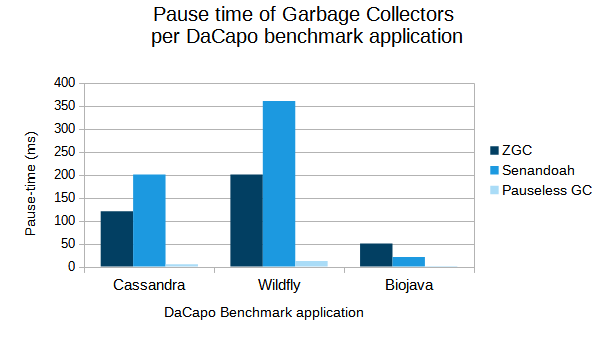
\includegraphics[width=1\columnwidth]{img/graph2.png}
    \end{figure}
\end{graph1section}


\begin{graph2section}
%    \caption{Simulatie van verwachte resultaten van de gebruikte geheugen op piekmoment voor bepaalde Garbage Collectors voor enkele DaCapo benchmark applicaties:}
    \begin{figure}[hbt!]
        \centering
        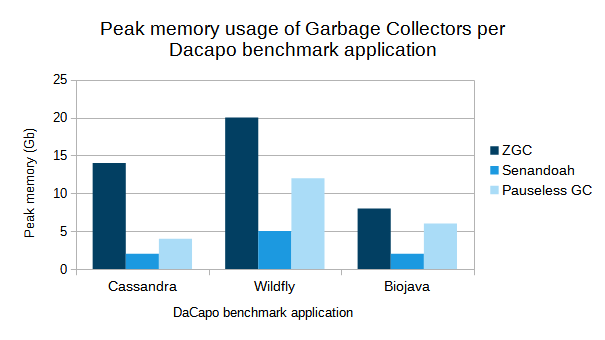
\includegraphics[width=1\columnwidth]{img/graph3.png}
    \end{figure}
\end{graph2section}
%Hier beschrijf je welke resultaten je verwacht. Als je metingen en simulaties uitvoert, kan je hier al mock-ups maken van de grafieken samen met de verwachte conclusies. Benoem zeker al je assen en de onderdelen van de grafiek die je gaat gebruiken. Dit zorgt ervoor dat je concreet weet welk soort data je moet verzamelen en hoe je die moet meten.

%Wat heeft de doelgroep van je onderzoek aan het resultaat? Op welke manier zorgt jouw bachelorproef voor een meerwaarde?

%Hier beschrijf je wat je verwacht uit je onderzoek, met de motivatie waarom. Het is \textbf{niet} erg indien uit je onderzoek andere resultaten en conclusies vloeien dan dat je hier beschrijft: het is dan juist interessant om te onderzoeken waarom jouw hypothesen niet overeenkomen met de resultaten.



\printbibliography[heading=bibintoc]

\end{document}